\chapter{Introducción}

El presente documento corresponde a la realización de un Trabajo Final del Grado en Electrónica Industrial y Automática basado en la conexión e integración de un brazo robótico en una red domótica. A continuación, se recoge de manera ordenada y detallada el desarrollo e implementación del proyecto; así como los resultados obtenidos y las conclusiones a kas que es posible llegar.

\section{Motivación del proyecto}

El punto de partida es el proyecto Robohealth. Consiste en un conjunto de entidades en colaboración para el desarrollo de soluciones relacionadas con la robótica y la domótica con el fin de introducir mejoras en el sistema sanitario. Como se puede observar, entre estas entidades está, además de otras dos universidades públicas de la Comunidad de Madrid, la Universidad Politécnica de Madrid.

Los resultados del proyecto están orientados a pacientes con enfermedades crónicas o capacidades cognitivas limitadas, pacientes en una situación de dependencia a los que es posible mejorar la calidad de vida. Estas mejoras se obtienen a través del diseño y fabricación de robots de asistencia, tanto para pacientes como para sus cuidadores, y la implementación de entornos inteligentes.

En la figura \ref{fig:RH}, se pueden observar los diferentes paquetes de trabajo y subproyectos en los que se trabaja dentro de la estructura de RoboHealth, repartidos entre las entidades colaboradoras. En la Universidad Politécnica de Madrid, encargada del desarrollo de entornos inteligentes de asistencia y rehabilitación, se ha venido trabajando en distintas herramientas enmarcadas en Trabajos Finales de Grado durante los últimos años.

\begin{figure}[tb]
\centering
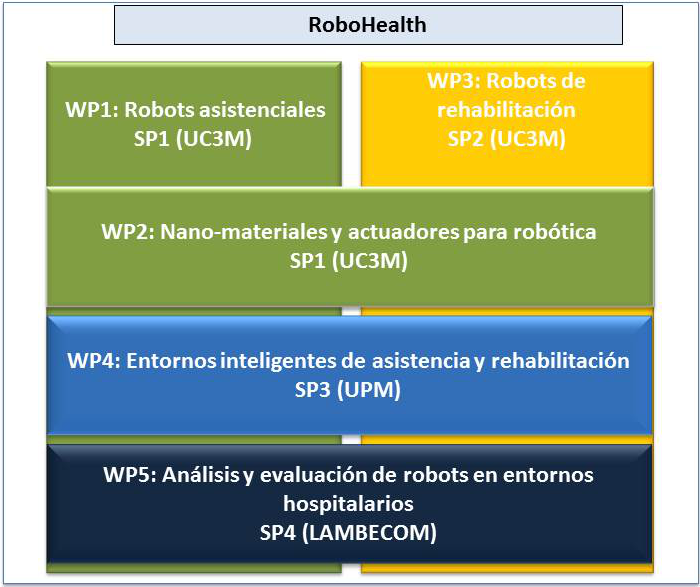
\includegraphics[width=0.55\textwidth]{figuras/RHstruct.png}
\caption{Estructura RoboHealth}
\label{fig:RH}
\end{figure}

Dentro del marco previamente expuesto, se han desarrollado dos plataformas que sirven de base para el proyecto objetivo de este documento.

\begin{itemize}
\item \textbf{RoboHealth Arm} es un brazo robótico de tres grados de libertad (actualmente, cuenta con sólo dos grados de libertad operativos) diseñado para sustentar una tablet en su extremo, haciendo más acesible su uso para pacientes y cuidadores. Está basado en un sitema de cuerdas y poleas accionado por tres servomotores.
\item Por otro lado, existe una aplicacion de \textbf{Node-RED} que integra los diferentes dispositivos y proyectos desarrollados en una red domótica. Incluye una interfaz gráfica que facilita su interacción vía internet, posibilitando controlar los dispositivos desde cualquier lugar.
\end{itemize} 

La idea es continuar el proceso de integración de los diferentes dispositivos en Node-RED con la intención de controlar todo desde la misma interfaz. En ese contexto, surge el proyecto de hacerlo con el brazo RoboHealth Arm. Con el fin de tratar de explorar todas las tecnologías posibles, se comprueba que la radiofrecuencia aún no habia sido y existen soluciones económicas en el mercado.

Así, el planteamient del Trabajo Final de Grado tomó forma, defiendose como la conexión mediante el uso de radiofrecuencia del brazo RoboHealth Arm a la interfaz de Node-RED. Para la radiofrecuencia, se usarán dispositivos XBee.

\section{Objetivos}\label{sec:refobj}

Como se ha indicado con anterioridad, el \textbf{objetivo global} del proyecto es la completa integración de un control a través de internet del brazo robótico. Los comandos se lanzan desde la interfaz de Node-Red y el ordenador de la sala transmite la orden vía radiofrecuencia al brazo.

Posteriormente, se pueden establecer pequeños \textbf{objetivos parciales} que resulten en la consecución completa del proyecto. Estos objetivos secundarios están más orientados al correcto funcionamiento de cada una de las etapas y tecnologías utilizadas, así como de la correcta interacción entre estas y su posterior integración. Es este el procedimiento que se ha seguido a lo largo de todo el trabajo: hacer funcionar cada etapa de manera individual, para después ir integrándolas paso a paso.

Los objetivos parciales mencionados son los siguientes, yendo desde el lado de Node-RED hacia el lado del RoboHealth Arm:

\begin{itemize}

\item Un programa de flujos en Node-RED debe correr sin errores en la Raspberry Pi, generando un nuevo apartado en la actual interfaz para controlar el RoboHealth Arm.

\item Desarrollar una \textit{user interface} para comandar el brazo desde Node-RED. El objetivo no es otro que permitir configurar las coordenadas articulares del brazo, parámetros necesarios en el frame que posteriormente deberá recibir el RoboHealth Arm. Una vez configurados, se tendrá acceso a un botón encargado de poner en marcha la transmisión de información.

\item La orden enviada desde la interfaz de Node-RED pondrá en marcha un script programado en Python que tomará como parámetros la configuración previamente establecida y enviará por uno de los puertos serie el frame generado de acuerdo a las especificaciones de diseño de la comunicación del RoboHealth Arm y el encapsulamiento de las comunicaciones vía radiofrecuencia. Toda la gestión de la ejecución de este script ha sido programada en Node-RED.

\item El firmware cargado a los dispositivos XBee debe hacerlos compatibles entre ellos, de acuerdo a las características y casos de uso a los que cada uno se va a enfrentar.

\item La configuración de los módulos XBee es vital para su comunicación. Esta configuración debe habilitar la comunicación entre los dos dispositivos XBee sin dejar de permitir la comunicación serial con el RoboHealth Arm ni con la Raspberry Pi. Es decir, los módulos XBee deben ser configurados de tal manera que esta configuración sea intersección entre la compatible con el brazo robótico y la compatible con la Raspberry Pi.

\item Un dispositivo XBee ha sido configurado para enviar el frame de datos recibido por comunicación serial. Al poder concentrarse todo el procesamiento de la información correspondiente al emisor en el anteriormente mencionado script, no se precisa de ningún microcontrolador adicional que funcione junto al módulo de radiofrecuencia. Así pues, el módulo XBee funciona de manera exclusiva como un traductor entre la información en el puerto serie correspondiente y las ondas de radiofrecuencia.

\item El dispositivo XBee receptor de la información que comanda el brazo robótico esta situado en el mismo. Su objetivo es ser capaz de captar el mensaje de radio específicamente diseñado para él y transmitirlo al microcontrolador del brazo. De la misma manera que en el otro XBee, su función será la de traductor de las ondas de radio (excusivamente de las destinadas a él) en información en el puerto serial. Por tanto, no es necesario procesar en ningún caso la información recibida a traves de radiofrecuencia, evitando un segundo microcontrolador que escuche y adapte constantemente el módulo XBee. Esto es posible gracias al prediseño de los frames de información de acuerdo a las especificaciones y protocolos de comunicación del brazo. 

\item El RoboHealth Arm debe ser capaz de leer e interpretar de manera correcta la información depositada en el adecuado puerto serial. Se debe provocar la reacción esperada en el brazo, moviendo sus servos hasta las coordenadas articulares especificadas.

\end{itemize}


\section{Materiales utilizados}

Con el fin de facilitar al lector una visión global de los campos objeto del presente proyecto, a continuación se indican los componentes del mismo.

\subsection{Componentes hardware}
\begin{itemize}
\item \textbf{Raspberry Pi 3 Model B} (figura \ref{fig:RPi3}). Ordenador central donde corre la red domótica de toda la habitación

\begin{figure}[H]
\centering
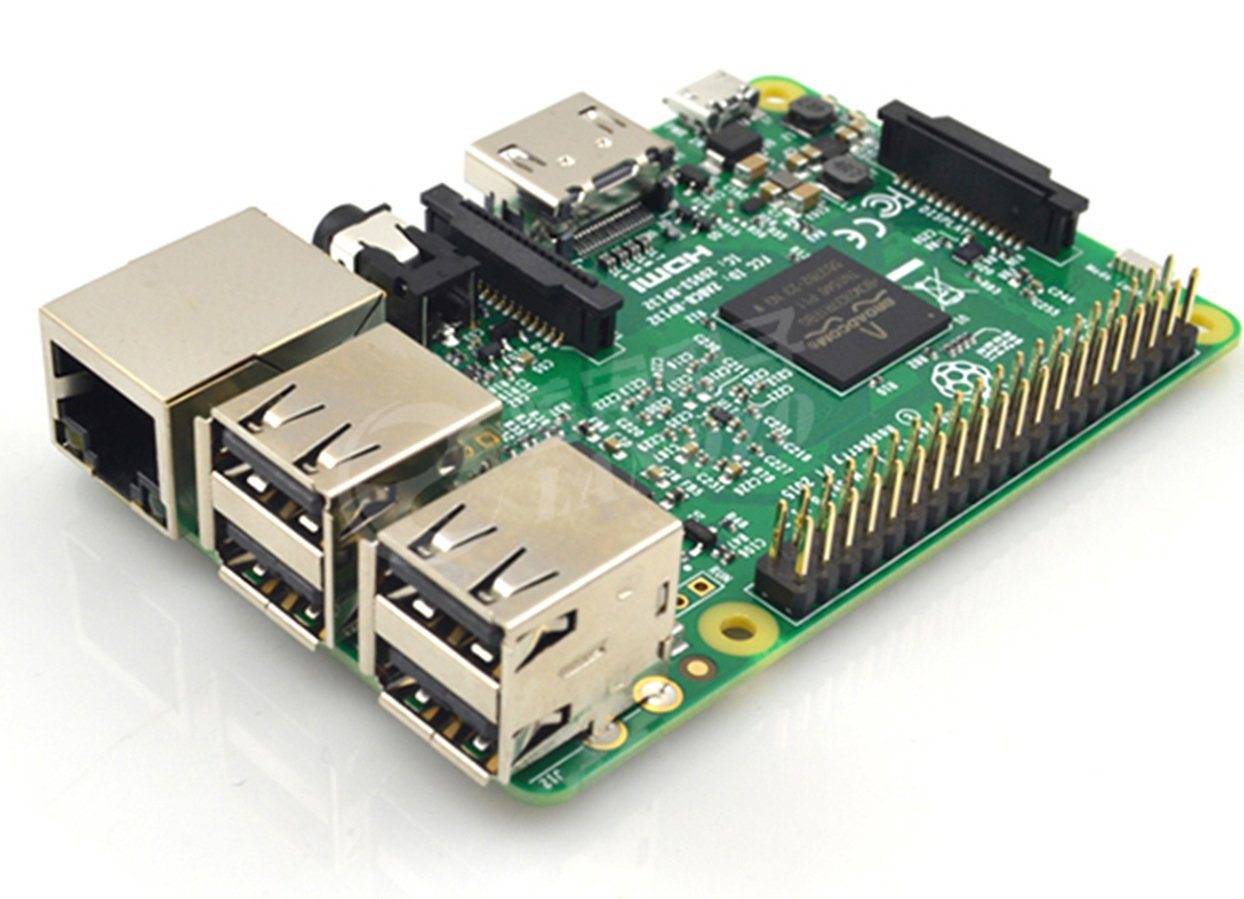
\includegraphics[width=0.45\textwidth]{figuras/RPi3.png}
\caption{Raspberry Pi 3 model B}
\label{fig:RPi3}
\end{figure}

\item \textbf{Arduino Uno R3} o clon (figura \ref{fig:AUno}). Plataforma necesaria para el uso de la XBee Shield.

\begin{figure}[H]
\centering
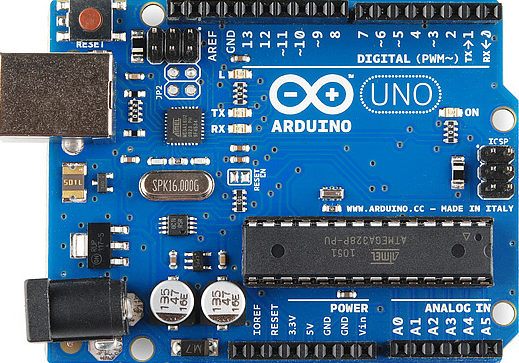
\includegraphics[width=0.45\textwidth]{figuras/AUno.png}
\caption{Arduino Uno R3}
\label{fig:AUno}
\end{figure}

\item \textbf{Xbee Shield} (figura \ref{fig:XBeeSh} \footnote{La imagen contiene el módulo XBee además de la XBee Shield}). \textit{Add-on} que permite la interacción sencilla con el módulo XBee a través de Arduino.

\begin{figure}[H]
\centering
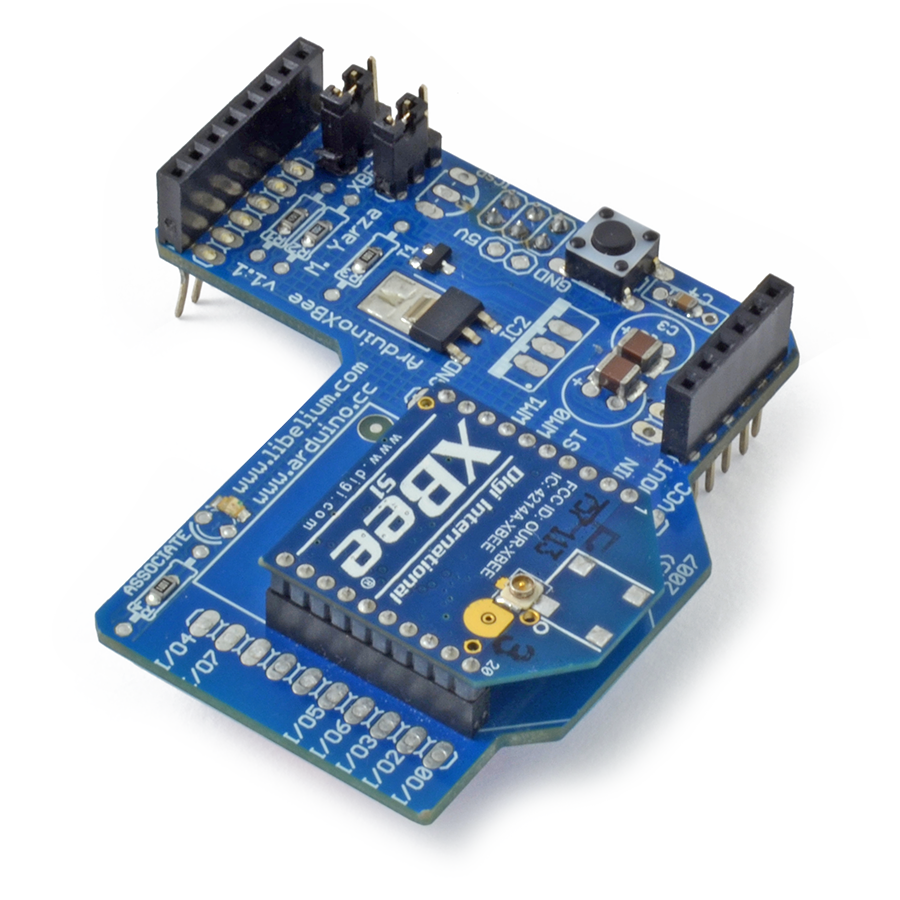
\includegraphics[width=0.45\textwidth]{figuras/XBeeShield.png}
\caption{XBee Shield}
\label{fig:XBeeSh}
\end{figure}

\item \textbf{XBee S2} (figura \ref{fig:Xbee}). Módulo de radiofrecuencia para la transmision inalámbrica de datos

\begin{figure}[H]
\centering
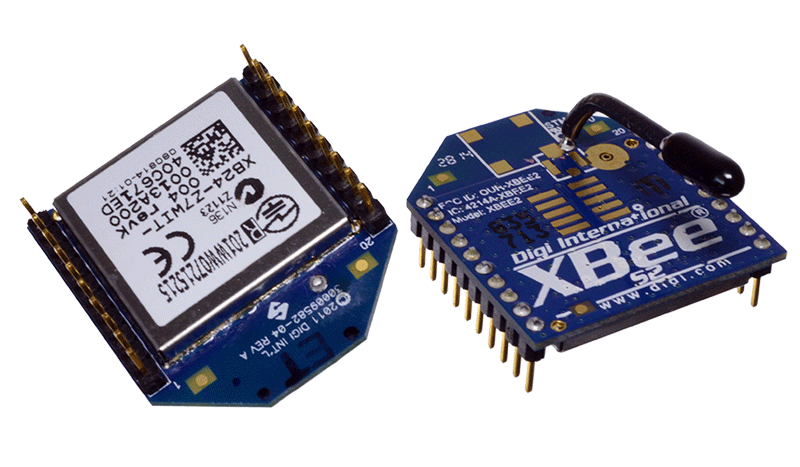
\includegraphics[width=0.45\textwidth]{figuras/XBee.png}
\caption{XBee Module}
\label{fig:Xbee}
\end{figure}

\item \textbf{Arduino Mega} (figura \ref{fig:AMega}). Microcontrolador sobre le que se monta RoboHealth Arm.

\begin{figure}[H]
\centering
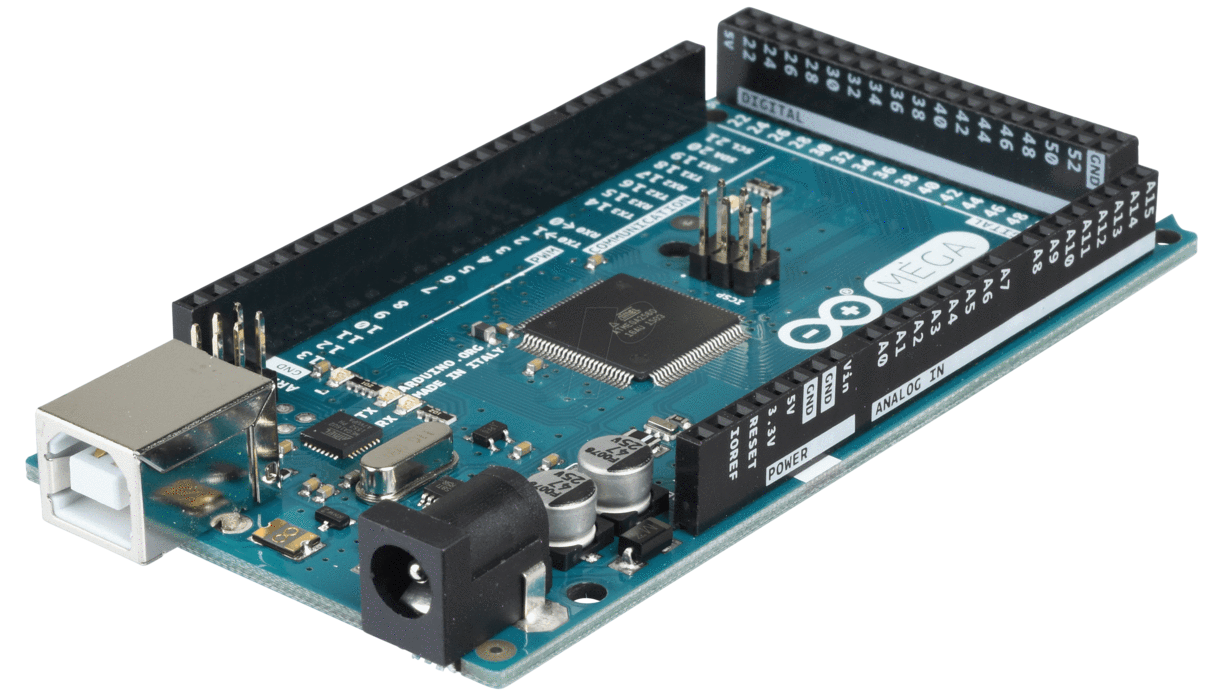
\includegraphics[width=0.45\textwidth]{figuras/AMega.png}
\caption{Arduino Mega}
\label{fig:AMega}
\end{figure}

\end{itemize}

\subsection{Componentes software}
\begin{itemize}
\item \textbf{Raspbian}. Sistema operativo instalado sobre la Raspberry Pi.
\item \textbf{Python script}. Programa escrito en lenguaje Phyton para ser ejecutado por la Raspberry Pi.
\item \textbf{Node-RED} (figura \ref{fig:NodeRED}). Aplicación programable que es capaz de integrar múltiples dispositivos hardware.

\begin{figure}[H]
\centering
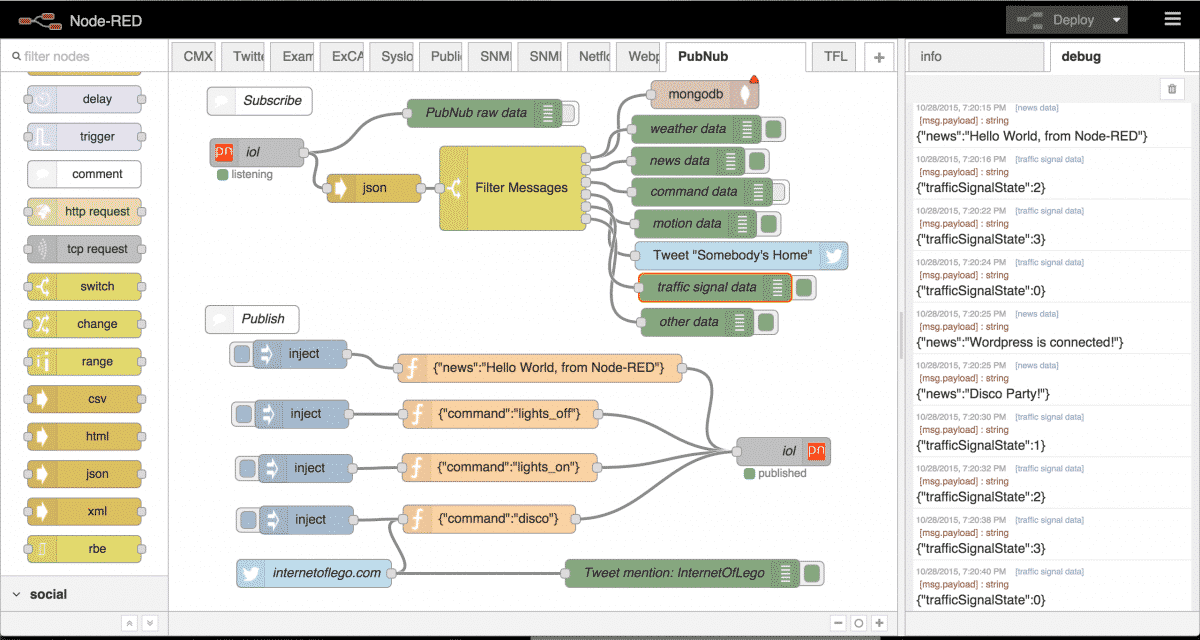
\includegraphics[width=0.45\textwidth]{figuras/NodeRED.png}
\caption{Interfaz de edición de Node-RED}
\label{fig:NodeRED}
\end{figure}

\item \textbf{RHA}. Software del RoboHealth Arm.

\end{itemize}

\section{Estructura del documento}

A continuación, y para facilitar la lectura del documento, se detalla el contenido de cada capítulo.

\begin{itemize}
\item En el capítulo 1 se realiza una introducción al proyecto. Un breve comentario sobre la idea y componentes del trabajo.
\item En el capítulo 2 se exponen los fundamentos teóricos que pueden facilitar la lectura posterior del desarrollo del proyecto.
\item En el capítulo 3 se encuenta el estado del arte, un repaso a la tecnología actualmente desarrollada incluida en el proyecto, para conocer con mayor precisión el punto de partida del mismo.
\item En el capítulo 4 se detalla el desarrollo del trabajo. Se exploran las soluciones hardware, software, montaje...
\item En el capítulo 5 se exponen y discuten las pruebas y los resultados del proyecto.
\item En el capítulo 6 se describe la gestion del proyecto; incluyendo la planificación, el presupuesto, ciclo de vida...
\item Para finalizar, en el capítulo 7 se termina con las conclusiones sacadas del proyecto y potenciales desarrollos futuros.
\end{itemize}
